\section{Caractérisation des matériaux}
\begin{enumerate}
  \item \q{Ecrire une fonction }\il{transf(d, f)}\q{ qui prend en argument un allongement et une force, et qui retourne deux valeurs :}
        \begin{itemize}
          \item \il{eps} \q{, la valeur de l'allongement relatif}
          \item \il{sigma} \q{la valeur de la contrainte}
        \end{itemize}
        Pour une meilleure organisation, je crée un dossier \il{ressources} dans lequel je placerais toutes les ressources.
        Pour l'instant je crée le fichier \il{ressources/donnees.py} :
        \codeFromFile{section-02/q1-1.py}
        J'importe les librairies qui me seront utiles plus tard :
        \codeFromFile{section-02/q1-2.py}
        Je peux maintenant répondre à la question :
        \codeFromFile{section-02/q1-3.py}

  \item \q{Ecrire une fonction }\il{lecture(essai)}\q{ qui prend en argument le nom de l'essai, et qui retourne :}
        \begin{itemize}
          \item \q{Le nom du matériau de l'essai}
          \item \q{Un tableau à 2 colonnes composées uniquement de données numériques :}
                \begin{itemize}
                  \item \q{La $1^{\grave{e}re}$ indiquant les allongements relatifs de l'essai}
                  \item \q{La $2^{\grave{e}me}$ indiquant les contraintes correspondantes à celles des allongements relatifs.}
                \end{itemize}
        \end{itemize}
        Je place les 4 résultats des essais \il{essai_1.csv}, \il{essai_2.csv}, \il{essai_3.csv} et \il{essai_4.csv} dans le dossier \il{ressources}.
        Je préfère décomposer la question en plusieurs fonctions :

        \codeFromFile{section-02/q2-1.py}

        Le classique \il{isNumeric} qui n'existe pas simplement en Python !

        \codeFromFile{section-02/q2-2.py}
        \il{clearEmptyCells} pour supprimer d'éventuelles cellules vides.

        Et enfin :
        \codeFromFile{section-02/q2-3.py}


  \item \q{Ecrire une procédure }\il{trace(nom, T)}\q{ qui prend en argument le nom du matériau, et un tableau à 2 colonnes de données numériques et qui trace la colonne
          1 en fonction de la colonne 1 avec pour légende le nom du matériau et :}
        \begin{itemize}
          \item \q{Pour titre : "Essais de traction"}
          \item \q{Pour label d'abscisse : "Allongement relatif"}
          \item \q{Pour label d'ordonnée : "Contrainte (MPa)"}
          \item \q{La légende affichée au milieu à gauche de la figure}
        \end{itemize}
        \codeFromFile{section-02/q3.py}

  \item \q{Ecrire une procédure }\il{figure(n)}\q{ qui prend en argument le nombre d'essai }\il{n}\q{ à tracer, et qui les trace sur la même figure.}
        \codeFromFile{section-02/q4.py}
        J'ai déplacé la légende à droite, car elle cachait les courbes.
        Voici le graphe obtenu :
        \begin{center}
          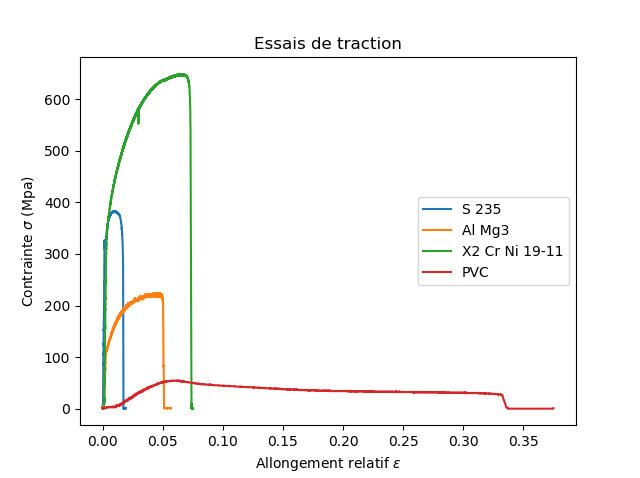
\includegraphics[scale=0.8]{section-02/q4.png}
        \end{center}


  \item \q{Ecrire une fonction }\il{rupture(T)}\q{ qui prend en argument un tableau à 2 colonnes $(\epsilon, \sigma)$ et qui retourne la valeur de la limite à la rupture $R_m$.}
        Vu comme j'ai codé les fonctions précédentes, il faut que cette fonction prenne directement la liste des $\sigma$ en paramètre :
        \codeFromFile{section-02/q5-1.py}
        En exécutant :
        \codeFromFile{section-02/q5-2.py}
        On trouve :
        \il{382.6092} Mpa


  \item \q{Ecrire une fonction }\il{select(T)}\q{ qui prend en argument les données issues de l'essai et qui retourne la partie du tableau qui correspond à la plage définie plus haut.}

        D'abord j'ai besoin d'une petite fonction de recherche :
        \codeFromFile{section-02/q6-1.py}
        Puis je code la fonction demandée :
        \codeFromFile{section-02/q6-2.py}
        En traçant pour le premier essai en orange la plage sélectionnée, et en bleu toute les valeurs on a :
        \begin{center}
          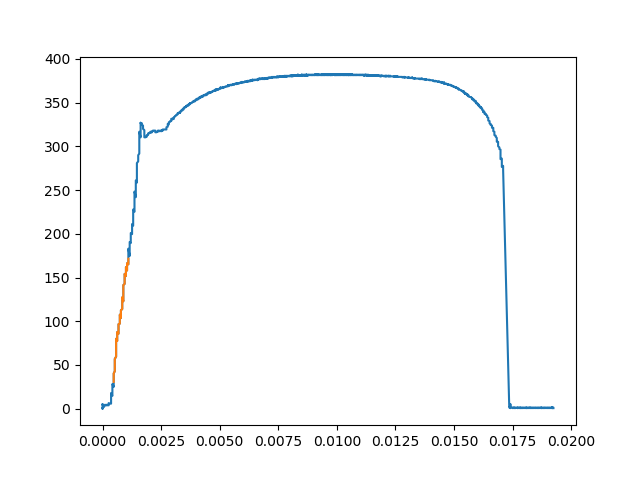
\includegraphics[scale=0.8]{section-02/q6-3.png}
        \end{center}


  \item \q{Ecrire une fonction }\il{somme(Ts)}\q{ qui prend en argument le tableau de données sélectionnées et qui retourne un tableau }\il{Som}\q{ dans lequel seront rangées les 5 valeurs }
        \il{Sxi}\q{, }
        \il{Syi}\q{, }
        \il{Sxiyi}\q{ et }
        \il{Sxi2}\q{ et }
        \il{n}\q{ pour la plage de données concernée.}
        \codeFromFile{section-02/q7.py}
        On obtient :
        \[
          \begin{array}{rcl}
            \il{Sxi}   & = & \il{0.07786759130836801}   \\
            \il{Syi}   & = & \il{10925.483200000002}    \\
            \il{Sxiyi} & = & \il{9.156426879112345}     \\
            \il{Sxi2}  & = & \il{6.375307483976406e-05} \\
            \il{n}     & = & \il{100}                   \\
          \end{array}
        \]


  \item \q{Ecrire une fonction }\il{Young(T)}\q{ qui prend en argument le tableau de données issues de l'essai de traction et qui retourne le module d'élasticité $E$ et la valeur initiale $sigm_0$ pour la plage de donnée concernée.}
        \codeFromFile{section-02/q8.py}

        On obtient :
        \[
          \begin{array}{rcl}
            \il{E}     & = & \il{208054.24028098426} \\
            \il{simg0} & = & \il{-52.75199352172678} \\
          \end{array}
        \]


  \item \q{Ecrire une fonction }\il{lim_el(T)}\q{ qui prend en argument les données issues de l'essai et qui retourne la limite élastique $R_e$.}

        Je définis d'abord une petite fonction test :
        \codeFromFile{section-02/q9-1.py}

        Puis je code la fonction demandée :
        \codeFromFile{section-02/q9-2.py}

        On obtient :
        \[
          \begin{array}{rcl}
            R_e & = & \il{161.8732} \\
          \end{array}
        \]

\end{enumerate}
